\documentclass{standalone}

\usepackage{graphicx}
\usepackage{subcaption}
\usepackage{tikz}
\usepackage{xcolor}
\usepackage{pgfplots}
\usepackage{etoolbox}
\usepgfplotslibrary{units,groupplots}

\definecolor{wblack}{RGB}{0, 0, 0}
\definecolor{worange}{RGB}{230, 159, 0}
\definecolor{wskyblue}{RGB}{86, 180, 233}
\definecolor{wgreen}{RGB}{0, 158, 115}
\definecolor{wyellow}{RGB}{240, 228, 66}
\definecolor{wblue}{RGB}{0, 114, 178}
\definecolor{wred}{RGB}{213, 94, 0}
\definecolor{wpurple}{RGB}{204, 121, 167}

\pgfplotsset{
    compat=newest,
    width=6cm,
    height=22mm,
    scale only axis=true,
    scaled ticks=false,
    xticklabel style={/pgf/number format/fixed},
    xlabel shift=-4pt,
    %max space between ticks=25pt,
    %try min ticks=5,
    %every axis plot/.append style={thick},
    %tick style={black, thick}
}
\usepackage{etoolbox}

\newcommand{\addPlotIfExists}[3]{%
    \begingroup
    \IfFileExists{#2}{%
        \addplot [#1] table [x=fraction, y=speedup, col sep=comma] {#2};
        \addlegendentry{#3}
    }{}
    \endgroup
}

\begin{document}

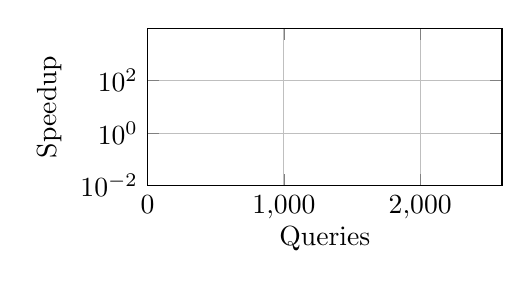
\begin{tikzpicture}
\begin{axis}[
    width=45mm,   % shrink plot so legend fits right
    height=2cm,
    xlabel={Queries},
    ylabel={Speedup},
    ymode=log,
    grid=both,
    xmin=0,
    xmax=2600,
    ymin=1e-2,
    ymax=1e+4,
    ytick={1e-2, 1,1e2},
    %legend columns=1, % one single column
    legend cell align=left,
    legend style={
        at={(1.03,.35)},      % right of plot
        anchor=west,  % align top
        draw=none
    }
]

\addPlotIfExists {mark=none, wblack}    {bench/results/csv/ce/ablation/cdf_CodegenFlatLeftDeep_v.csv}              {Flat}
\addPlotIfExists {mark=none, wskyblue}  {bench/results/csv/ce/ablation/cdf_CodegenFactorizedLeftDeep_v.csv}        {Factorized}
\addPlotIfExists {mark=none, wblue}     {bench/results/csv/ce/ablation/cdf_CodegenFactorizedLeftDeep_vb.csv}       {+ bottom-insert}
\addPlotIfExists {mark=none, wpurple}   {bench/results/csv/ce/ablation/cdf_CodegenFactorizedLeftDeep_vbc.csv}      {+ caching}
\addPlotIfExists {mark=none, wred}      {bench/results/csv/ce/ablation/cdf_CodegenFactorizedLeftDeep_vbic.csv}     {+ inlining}
\addPlotIfExists {mark=none, worange}   {bench/results/csv/ce/ablation/cdf_CodegenFactorized_vbic.csv}             {+ bushy trees}
\addPlotIfExists {mark=none, wgreen}    {bench/results/csv/ce/ablation/cdf_CodegenFactorizedLeftDeep_pvbic.csv}    {+ parallel}

\end{axis}
\end{tikzpicture}

\end{document}